\documentclass[11pt,letterpaper,notitlepage]{article}
\usepackage[left=1in,right=1in,top=1in,bottom=1in]{geometry}
\usepackage[dvipsnames]{xcolor}
\definecolor{darkblue}{RGB}{46,48,147}
\usepackage{hyperref}
\hypersetup{colorlinks=true,
            linkcolor=darkblue,
            urlcolor=darkblue,
            citecolor=darkblue}
\usepackage{xspace}
\usepackage{amsmath,amsfonts,amssymb}
\usepackage{lipsum}
\usepackage[utf8]{inputenc}
\usepackage[T1]{fontenc}
\usepackage{palatino}
\usepackage{mathpazo}
\usepackage{ifthen}
\newboolean{cms@italic}
\setboolean{cms@italic}{false}
\newboolean{cms@external}
\setboolean{cms@external}{false}
\usepackage[pazoGreek]{heppennames2}
\usepackage{ptdr-definitions}
\usepackage{lastpage}
\usepackage{fancyhdr}
\usepackage{graphicx}
\renewcommand{\headrulewidth}{0pt}
\lhead{Javier M. Duarte}
\rhead{Personal Statement}
\cfoot{\thepage}

\newcommand{\mycite}[1]{%
\ifthenelse{\equal{#1}{Khachatryan:2015pwa}}{\href{https://doi.org/10.1103/PhysRevD.91.052018}{\textbf{A.I.277}}}{}%
\ifthenelse{\equal{#1}{Anderson:2015tia}}{\href{https://doi.org/10.1016/j.nima.2014.11.041}{\textbf{A.I.311}}}{}%
\ifthenelse{\equal{#1}{Anderson:2015gha}}{\href{https://doi.org/10.1016/j.nima.2015.04.013}{\textbf{A.I.317}}}{}%
\ifthenelse{\equal{#1}{Anderson:2016ygg}}{\href{https://doi.org/10.1109/TNS.2016.2528166}{\textbf{A.I.373}}}{}%
\ifthenelse{\equal{#1}{Anderson:2016tiu}}{\href{https://doi.org/10.1016/j.nima.2015.11.129}{\textbf{A.I.396}}}{}%
\ifthenelse{\equal{#1}{Khachatryan:2016epu}}{\href{https://doi.org/10.1103/PhysRevD.95.012003}{\textbf{A.I.444}}}{}%
\ifthenelse{\equal{#1}{Sirunyan:2016iap}}{\href{https://doi.org/10.1016/j.physletb.2017.02.012}{\textbf{A.I.491}}}{}%
\ifthenelse{\equal{#1}{Sirunyan:2017nvi}}{\href{https://doi.org/10.1007/JHEP01(2018)097}{\textbf{A.I.567}}}{}%
\ifthenelse{\equal{#1}{Sirunyan:2017dgc}}{\href{https://doi.org/10.1103/PhysRevLett.120.071802}{\textbf{A.I.571}}}{}%
\ifthenelse{\equal{#1}{Sirunyan:2017eie}}{\href{https://doi.org/10.1016/j.physletb.2017.12.069}{\textbf{A.I.604}}}{}%
\ifthenelse{\equal{#1}{Duarte:2018ite}}{\href{https://doi.org/10.1088/1748-0221/13/07/P07027}{\textbf{A.I.644}}}{}%
\ifthenelse{\equal{#1}{Sirunyan:2018xlo}}{\href{https://doi.org/10.1007/JHEP08(2018)130}{\textbf{A.I.662}}}{}%
\ifthenelse{\equal{#1}{Sirunyan:2018kst}}{\href{https://doi.org/10.1103/PhysRevLett.121.121801}{\textbf{A.I.667}}}{}%
\ifthenelse{\equal{#1}{Sirunyan:2018ikr}}{\href{https://doi.org/10.1103/PhysRevD.99.012005}{\textbf{A.I.713}}}{}%
\ifthenelse{\equal{#1}{Sirunyan:2018koj}}{\href{https://doi.org/10.1140/epjc/s10052-019-6909-y}{\textbf{A.I.761}}}{}%
\ifthenelse{\equal{#1}{Sirunyan:2018sgc}}{\href{https://doi.org/10.1016/j.physletb.2019.03.059}{\textbf{A.I.762}}}{}%
\ifthenelse{\equal{#1}{Duarte:2019fta}}{\href{https://doi.org/10.1007/s41781-019-0027-2}{\textbf{A.I.794}}}{}%
\ifthenelse{\equal{#1}{Sirunyan:2019vxa}}{\href{https://doi.org/10.1103/PhysRevD.100.112007}{\textbf{A.I.817}}}{}%
\ifthenelse{\equal{#1}{Sirunyan:2019sgo}}{\href{https://doi.org/10.1103/PhysRevLett.123.231803}{\textbf{A.I.818}}}{}%
\ifthenelse{\equal{#1}{Moreno:2019bmu}}{\href{https://doi.org/10.1140/epjc/s10052-020-7608-4}{\textbf{A.I.824}}}{}%
\ifthenelse{\equal{#1}{Summers:2020xiy}}{\href{https://doi.org/10.1088/1748-0221/15/05/p05026}{\textbf{A.I.861}}}{}%
\ifthenelse{\equal{#1}{Sirunyan:2019vgj}}{\href{https://doi.org/10.1007/JHEP05(2020)033}{\textbf{A.I.866}}}{}%
\ifthenelse{\equal{#1}{Sirunyan:2019pnb}}{\href{https://doi.org/10.1016/j.physletb.2020.135448}{\textbf{A.I.875}}}{}%
\ifthenelse{\equal{#1}{Moreno:2019neq}}{\href{https://doi.org/10.1103/PhysRevD.102.012010}{\textbf{A.I.877}}}{}%
\ifthenelse{\equal{#1}{DiGuglielmo:2020eqx}}{\href{https://doi.org/10.1088/2632-2153/aba042}{\textbf{A.I.910}}}{}%
\ifthenelse{\equal{#1}{Sirunyan:2020hwz}}{\href{https://doi.org/10.1007/JHEP12(2020)085}{\textbf{A.I.911}}}{}%
\ifthenelse{\equal{#1}{Iiyama:2020wap}}{\href{https://doi.org/10.3389/fdata.2020.598927}{\textbf{A.I.915}}}{}%
\ifthenelse{\equal{#1}{Krupa:2020bwg}}{\href{https://doi.org/10.1088/2632-2153/abec21}{\textbf{A.I.930}}}{}%
\ifthenelse{\equal{#1}{Pata:2021oez}}{\href{https://doi.org/10.1140/epjc/s10052-021-09158-w}{\textbf{A.I.939}}}{}%
\ifthenelse{\equal{#1}{Aarrestad:2021zos}}{\href{https://doi.org/10.1088/2632-2153/ac0ea1}{\textbf{A.I.944}}}{}%
\ifthenelse{\equal{#1}{Hawks:2021ruw}}{\href{https://doi.org/10.3389/frai.2021.676564}{\textbf{A.I.948}}}{}%
\ifthenelse{\equal{#1}{DiGuglielmo:2021ide}}{\href{https://doi.org/10.1109/TNS.2021.3087100}{\textbf{A.I.951}}}{}%
\ifthenelse{\equal{#1}{John:2020sak}}{\href{https://doi.org/10.1103/PhysRevAccelBeams.24.104601}{\textbf{A.I.971}}}{}%
\ifthenelse{\equal{#1}{Dezoort:2021kfk}}{\href{https://doi.org/10.1007/s41781-021-00073-z}{\textbf{A.I.974}}}{}%
\ifthenelse{\equal{#1}{Zlokapa:2019tkn}}{\href{https://doi.org/10.1007/s42484-021-00054-w}{\textbf{A.I.975}}}{}%
\ifthenelse{\equal{#1}{CMS:2021juv}}{\href{https://doi.org/10.1103/PhysRevLett.127.261804}{\textbf{A.I.987}}}{}%
\ifthenelse{\equal{#1}{Kasieczka:2021xcg}}{\href{https://doi.org/10.1088/1361-6633/ac36b9}{\textbf{A.I.988}}}{}%
\ifthenelse{\equal{#1}{Aarrestad:2021oeb}}{\href{https://doi.org/10.21468/SciPostPhys.12.1.043}{\textbf{A.I.992}}}{}%
\ifthenelse{\equal{#1}{Chen:2021euv}}{\href{https://doi.org/10.1038/s41597-021-01109-0}{\textbf{A.I.993}}}{}%
\ifthenelse{\equal{#1}{Govorkova:2021utb}}{\href{https://doi.org/10.1038/s42256-022-00441-3}{\textbf{A.I.994}}}{}%
\ifthenelse{\equal{#1}{Jawahar:2021vyu}}{\href{https://doi.org/10.3389/fdata.2022.803685}{\textbf{A.I.996}}}{}%
\ifthenelse{\equal{#1}{Elabd:2021lgo}}{\href{https://doi.org/10.3389/fdata.2022.828666}{\textbf{A.I.1004}}}{}%
\ifthenelse{\equal{#1}{CMS:2021yhb}}{\href{https://doi.org/10.1007/JHEP03(2022)160}{\textbf{A.I.1006}}}{}%
\ifthenelse{\equal{#1}{CMS:2022nmn}}{\href{https://doi.org/10.1103/PhysRevLett.131.041803}{\textbf{A.I.1028}}}{}%
\ifthenelse{\equal{#1}{CMS:2022dwd}}{\href{https://doi.org/10.1038/s41586-022-04892-x}{\textbf{A.I.1029}}}{}%
\ifthenelse{\equal{#1}{Touranakou:2022qrp}}{\href{https://doi.org/10.1088/2632-2153/ac7c56}{\textbf{A.I.1030}}}{}%
\ifthenelse{\equal{#1}{Kansal:2022spb}}{\href{https://doi.org/10.1103/PhysRevD.107.076017}{\textbf{A.I.1046}}}{}%
\ifthenelse{\equal{#1}{Bhimij:2022xyn}}{\href{https://doi.org/10.1007/s41781-023-00097-7}{\textbf{A.I.1047}}}{}%
\ifthenelse{\equal{#1}{Hao:2022zns}}{\href{https://doi.org/10.1140/epjc/s10052-023-11633-5}{\textbf{A.I.1052}}}{}%
\ifthenelse{\equal{#1}{Huerta:2022kgj}}{\href{https://doi.org/10.1038/s41597-023-02298-6}{\textbf{A.I.1057}}}{}%
\ifthenelse{\equal{#1}{CMS:2022wqf}}{\href{https://doi.org/10.1103/PhysRevLett.131.041801}{\textbf{A.I.1073}}}{}%
\ifthenelse{\equal{#1}{CMS:2022wjc}}{\href{https://doi.org/10.1007/JHEP07(2023)210}{\textbf{A.I.1078}}}{}%
\ifthenelse{\equal{#1}{Kansal:2023joss}}{\href{https://doi.org/10.21105/joss.05789}{\textbf{A.I.1112}}}{}%
\ifthenelse{\equal{#1}{Orzari:2023zrh}}{\href{https://doi.org/10.1088/2632-2153/ad04ea}{\textbf{A.I.1113}}}{}%
\ifthenelse{\equal{#1}{Shenoy:2023ros}}{\href{https://doi.org/10.1088/2632-2153/ad1139}{\textbf{A.I.1126}}}{}%
\ifthenelse{\equal{#1}{Duarte:2022job}}{\href{https://doi.org/10.1088/2632-2153/ad12e3}{\textbf{A.I.1127}}}{}%
\ifthenelse{\equal{#1}{Weng:2023tailor}}{\href{https://doi.org/10.1145/3624990}{\textbf{A.I.1140}}}{}%
\ifthenelse{\equal{#1}{Black:2022cth}}{\href{https://doi.org/10.1088/1748-0221/19/02/T02015}{\textbf{A.I.1142}}}{}%
\ifthenelse{\equal{#1}{CMS:2024twn}}{\href{https://arxiv.org/abs/2402.15366}{\textbf{A.I.1144}}}{}%
\ifthenelse{\equal{#1}{CMS:2024bvl}}{\href{https://arxiv.org/abs/2402.01898}{\textbf{A.I.1145}}}{}%
\ifthenelse{\equal{#1}{Pata:2023rhh}}{\href{https://doi.org/10.1038/s42005-024-01599-5}{\textbf{A.I.1155}}}{}%
\ifthenelse{\equal{#1}{CMS:2023gfb}}{\href{https://doi.org/10.1088/1748-0221/19/05/P05064}{\textbf{A.I.1158}}}{}%
\ifthenelse{\equal{#1}{Campos:2023pkp}}{\href{https://doi.org/10.1145/3662000}{\textbf{A.I.1168}}}{}%
\ifthenelse{\equal{#1}{Weng:2024fkeras}}{\href{https://doi.org/10.1145/3665334}{\textbf{A.I.1178}}}{}%
\ifthenelse{\equal{#1}{CMS:2024ake}}{\href{https://doi.org/10.1103/PhysRevD.110.012004}{\textbf{A.I.1181}}}{}%
\ifthenelse{\equal{#1}{Odagiu:2024bkp}}{\href{https://doi.org/10.1088/2632-2153/ad5f10}{\textbf{A.I.1183}}}{}%
\ifthenelse{\equal{#1}{Deiana:2021niw}}{\href{https://doi.org/10.3389/fdata.2022.787421}{\textbf{A.II.1}}}{}%
\ifthenelse{\equal{#1}{Duarte:2022efficient}}{\href{https://doi.org/10.3389/frai.2022.999173}{\textbf{A.II.2}}}{}%
\ifthenelse{\equal{#1}{Duarte:2020ngm}}{\href{https://doi.org/10.1142/9789811234033_0012}{\textbf{A.III.1}}}{}%
\ifthenelse{\equal{#1}{neurips2019_sonic}}{\href{https://doi.org/10.5281/zenodo.3895029}{\textbf{A.IV.1}}}{}%
\ifthenelse{\equal{#1}{neurips2019_hbb}}{\href{https://doi.org/10.5281/zenodo.3895048}{\textbf{A.IV.2}}}{}%
\ifthenelse{\equal{#1}{neurips2019_hls4ml}}{\href{https://doi.org/10.5281/zenodo.3895081}{\textbf{A.IV.3}}}{}%
\ifthenelse{\equal{#1}{Rankin:2020usv}}{\href{https://doi.org/10.1109/H2RC51942.2020.00010}{\textbf{A.IV.4}}}{}%
\ifthenelse{\equal{#1}{Heintz:2020soy}}{\href{https://arxiv.org/abs/2012.01563}{\textbf{A.IV.5}}}{}%
\ifthenelse{\equal{#1}{Kansal:2020svm}}{\href{https://arxiv.org/abs/2012.00173}{\textbf{A.IV.6}}}{}%
\ifthenelse{\equal{#1}{Fahim:2021cic}}{\href{https://arxiv.org/abs/2103.05579}{\textbf{A.IV.7}}}{}%
\ifthenelse{\equal{#1}{Orzari:2021suh}}{\href{https://arxiv.org/abs/2109.15197}{\textbf{A.IV.8}}}{}%
\ifthenelse{\equal{#1}{Mokhtar:2021bkf}}{\href{https://arxiv.org/abs/2111.12840}{\textbf{A.IV.9}}}{}%
\ifthenelse{\equal{#1}{Banbury:2021mlperf}}{\href{https://arxiv.org/abs/2106.07597}{\textbf{A.IV.10}}}{}%
\ifthenelse{\equal{#1}{Kansal:2021cqp}}{\href{https://arxiv.org/abs/2106.11535}{\textbf{A.IV.11}}}{}%
\ifthenelse{\equal{#1}{Tsan:2021brw}}{\href{https://arxiv.org/abs/2111.12849}{\textbf{A.IV.12}}}{}%
\ifthenelse{\equal{#1}{Pata:2022wam}}{\href{https://arxiv.org/abs/2203.00330}{\textbf{A.IV.13}}}{}%
\ifthenelse{\equal{#1}{Borras:2022opensource}}{\href{https://arxiv.org/abs/2206.11791}{\textbf{A.IV.14}}}{}%
\ifthenelse{\equal{#1}{Pappalardo:2022nxk}}{\href{https://arxiv.org/abs/2206.07527}{\textbf{A.IV.15}}}{}%
\ifthenelse{\equal{#1}{Duarte:2022hdp}}{\href{https://arxiv.org/abs/2207.07958}{\textbf{A.IV.16}}}{}%
\ifthenelse{\equal{#1}{Mokhtar:2022pwm}}{\href{https://arxiv.org/abs/2211.09912}{\textbf{A.IV.17}}}{}%
\ifthenelse{\equal{#1}{Hussain:2022faststamp}}{\href{https://doi.org/10.1145/3508352.3549357}{\textbf{A.IV.18}}}{}%
\ifthenelse{\equal{#1}{McDermott:2023neural}}{\href{https://arxiv.org/abs/2312.05978}{\textbf{A.IV.19}}}{}%
\ifthenelse{\equal{#1}{Mokhtar:2023fzl}}{\href{https://arxiv.org/abs/2303.17657}{\textbf{A.IV.20}}}{}%
\ifthenelse{\equal{#1}{Huang:2023bny}}{\href{https://arxiv.org/abs/2306.11330}{\textbf{A.IV.21}}}{}%
\ifthenelse{\equal{#1}{Amaro:2023voyager}}{\href{https://doi.org/10.1145/3569951.3597597}{\textbf{A.IV.22}}}{}%
\ifthenelse{\equal{#1}{Li:2023xhj}}{\href{https://arxiv.org/abs/2312.04757}{\textbf{A.IV.23}}}{}%
\ifthenelse{\equal{#1}{Miao:2024oqy}}{\href{https://arxiv.org/abs/2402.12535}{\textbf{A.IV.24}}}{}%
\ifthenelse{\equal{#1}{Baldi:2024reliable}}{\href{https://doi.org/10.1109/VTS60656.2024.10538639}{\textbf{A.IV.25}}}{}%
\ifthenelse{\equal{#1}{Duarte:2014soa}}{\href{https://arxiv.org/abs/1409.4466}{\textbf{B.I.1}}}{}%
\ifthenelse{\equal{#1}{Bornheim_2015}}{\href{https://doi.org/10.1088/1742-6596/587/1/012057}{\textbf{B.I.2}}}{}%
\ifthenelse{\equal{#1}{7581887}}{\href{https://doi.org/10.1109/NSSMIC.2015.7581887}{\textbf{B.I.3}}}{}%
\ifthenelse{\equal{#1}{Duarte:2016wnw}}{\href{https://doi.org/10.1016/j.nuclphysbps.2015.09.071}{\textbf{B.I.4}}}{}%
\ifthenelse{\equal{#1}{8069874}}{\href{https://doi.org/10.1109/NSSMIC.2016.8069874}{\textbf{B.I.5}}}{}%
\ifthenelse{\equal{#1}{Bornheim:2017gql}}{\href{https://doi.org/10.1088/1742-6596/928/1/012023}{\textbf{B.I.6}}}{}%
\ifthenelse{\equal{#1}{Duarte:2018bsd}}{\href{https://arxiv.org/abs/1808.00902}{\textbf{B.I.7}}}{}%
\ifthenelse{\equal{#1}{Albertsson:2018maf}}{\href{https://doi.org/10.1088/1742-6596/1085/2/022008}{\textbf{B.I.8}}}{}%
\ifthenelse{\equal{#1}{Aarrestad:2020ngo}}{\href{https://doi.org/10.5281/zenodo.4009114}{\textbf{B.I.9}}}{}%
\ifthenelse{\equal{#1}{Wozniak:2020}}{\href{https://doi.org/10.1051/epjconf/202024506039}{\textbf{B.I.10}}}{}%
\ifthenelse{\equal{#1}{Thais:2022iok}}{\href{https://arxiv.org/abs/2203.12852}{\textbf{B.I.11}}}{}%
\ifthenelse{\equal{#1}{Harris:2022qtm}}{\href{https://arxiv.org/abs/2203.16255}{\textbf{B.I.12}}}{}%
\ifthenelse{\equal{#1}{Apresyan:2022tqw}}{\href{https://arxiv.org/abs/2203.07353}{\textbf{B.I.13}}}{}%
\ifthenelse{\equal{#1}{Benelli:2022sqn}}{\href{https://arxiv.org/abs/2207.09060}{\textbf{B.I.14}}}{}%
\ifthenelse{\equal{#1}{Dawson:2022zbb}}{\href{https://arxiv.org/abs/2209.07510}{\textbf{B.I.15}}}{}%
\ifthenelse{\equal{#1}{Shanahan:2022ifi}}{\href{https://arxiv.org/abs/2209.07559}{\textbf{B.I.16}}}{}%
\ifthenelse{\equal{#1}{Agarwal:2023rwr}}{\href{https://arxiv.org/abs/2306.08106}{\textbf{B.I.17}}}{}%
\ifthenelse{\equal{#1}{Li:2024xpw}}{\href{https://doi.org/10.1051/epjconf/202429509017}{\textbf{B.I.18}}}{}%
\ifthenelse{\equal{#1}{Brigljevic:2024vuv}}{\href{https://arxiv.org/abs/2407.03015}{\textbf{B.I.19}}}{}%
\ifthenelse{\equal{#1}{Duarte:2017bbq}}{\href{https://arxiv.org/abs/1703.06544}{\textbf{B.IV.1}}}{}%
\ifthenelse{\equal{#1}{CMS-DP-2018-046}}{\href{https://cds.cern.ch/record/2630438}{\textbf{B.IV.2}}}{}%
\ifthenelse{\equal{#1}{CMS-PAS-EXO-17-026}}{\href{https://cds.cern.ch/record/2637847}{\textbf{B.IV.3}}}{}%
\ifthenelse{\equal{#1}{CERN-LHCC-2020-004}}{\href{https://cds.cern.ch/record/2714892}{\textbf{B.IV.4}}}{}%
\ifthenelse{\equal{#1}{hls4ml}}{\href{https://doi.org/10.5281/zenodo.1201549}{\textbf{B.IV.5}}}{}%
\ifthenelse{\equal{#1}{CMS-DP-2021-030}}{\href{https://cds.cern.ch/record/2792320}{\textbf{B.IV.6}}}{}%
\ifthenelse{\equal{#1}{CMS-PAS-HIG-21-012}}{\href{https://cds.cern.ch/record/2809929}{\textbf{B.IV.7}}}{}%
\ifthenelse{\equal{#1}{CMS-DP-2022-041}}{\href{https://cds.cern.ch/record/2839736}{\textbf{B.IV.8}}}{}%
\ifthenelse{\equal{#1}{CMS-DP-2022-061}}{\href{https://cds.cern.ch/record/2842375}{\textbf{B.IV.9}}}{}%
\ifthenelse{\equal{#1}{CMS-DP-2023-037}}{\href{https://cds.cern.ch/record/2863316}{\textbf{B.IV.10}}}{}%
\ifthenelse{\equal{#1}{CMS-PAS-HIG-21-020}}{\href{https://cds.cern.ch/record/2866501}{\textbf{B.IV.11}}}{}%
\ifthenelse{\equal{#1}{CMS-DP-2023-079}}{\href{https://cds.cern.ch/record/2876546}{\textbf{B.IV.12}}}{}%
\ifthenelse{\equal{#1}{Weng:2024architectural}}{\href{https://arxiv.org/abs/2403.08980}{\textbf{B.IV.13}}}{}%
\ifthenelse{\equal{#1}{CMS-PAS-HIG-23-012}}{\href{https://cds.cern.ch/record/2904879}{\textbf{B.IV.14}}}{}%
\ifthenelse{\equal{#1}{CMS-PAS-EXO-24-007}}{\href{https://cds.cern.ch/record/2904945}{\textbf{B.IV.15}}}{}%
}

\graphicspath{{PersonalStatement2022_figures/}}

\begin{document}

\pagestyle{fancyplain}

Below, I describe my contributions to research, teaching, mentorship, service, and equity, diversity and inclusion in the review period from June 30, 2022 to July 1, 2024.
\vspace{-1ex}
\subsection*{Research}

As an experimental particle physicist, my main research interests are to test the validity of the standard model (SM) of particle physics, our best theoretical description of elementary particles and their interactions, and search for signs of physics beyond the SM (BSM) in high-energy collision experiments.
To do this, I work as a collaborator on the CMS experiment at the CERN Large Hadron Collider (LHC), the world's most energetic particle collider.
The high energies of the LHC collisions allow us to probe the microscopic nature of subatomic particles on the smallest length scales: the higher the energy of the collisions, the smaller the length scale we can probe.
Much of my work studies high energy, or transverse momentum (\pt), particle production phenomena to probe nature at the shortest distance scales.

I analyze petabytes of proton-proton collision data to disentangle rare signal processes from the background to measure the properties and interactions of subatomic particles.
To enable this work, I develop algorithms based on artificial intelligence (AI) and machine learning (ML) to analyze the high-dimensional data from the detectors and classify or reconstruct particles or jets in these collision events.
My research focuses on
(R1) measurements of Higgs bosons decaying to quarks with \pt,
(R2) searches for exotic new physics involving jets and long-lived particles (LLPs),
(R3) developing novel AI and ML algorithms for event reconstruction and simulation to enable these physics results, and
(R4) developing methods to accelerate AI algorithm training and inference (i.e. execution), e.g., to improve the real-time LHC event selection in the trigger.
This work is naturally interdisciplinary, at the interface of physics, computer science, AI, and electrical engineering.
My research also crosses traditional academia/industry divides, and I have collaborated with computer scientists and engineers at Microsoft Research (e.g. Ted Way), AMD Adaptive and Embedded Computing Group (AECG) (formerly Xilinx Research, e.g. Michaela Blott), Intel Programmable Solutions Group (PSG) (e.g. Nabeel Shirazi), and Habana Labs.

\vspace{-1ex}
\subsubsection*{R1. High-\pt Higgs boson measurements}

On July 4, 2012, the discovery of a new fundamental particle, the Higgs boson (\PH), was announced by the ATLAS and CMS Collaborations.
This discovery confirmed the existence of a new kind of field, known as the Higgs field, whose physical incarnation is the Higgs boson.
Measuring the Higgs boson's interactions is necessary to confirm the validity of the SM, and any deviations may give a critical hint for new laws of physics.
To measure these interactions, we look for the Higgs boson in a multitude of production and decay processes, each one with a complementary sensitivity to a different set of couplings depending on the participating particles.
For example, measuring the rate of Higgs boson pair ($\PH\PH$) production enables us to constrain, and ultimately determine, the Higgs boson self-interaction strength $\lambda$ as well as the interaction strength between two vector bosons and two Higgs bosons $c_{2\PV}$.
This connection is illustrated in Fig.~\ref{fig:higgs}.

\begin{figure}[htb]
    \centering
    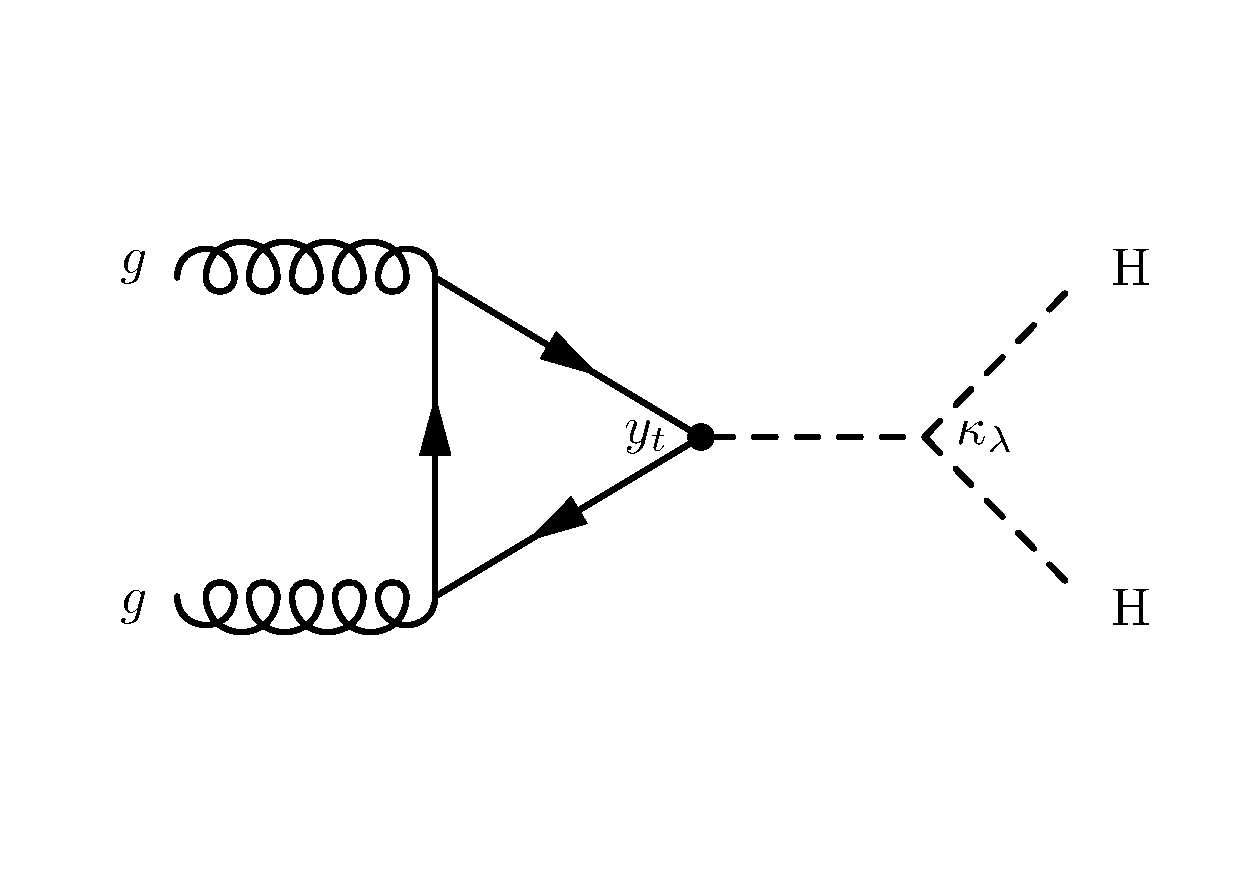
\includegraphics[width=0.45\textwidth]{CMS-PAS-HIG-23-012_Figure_001-a.pdf}
    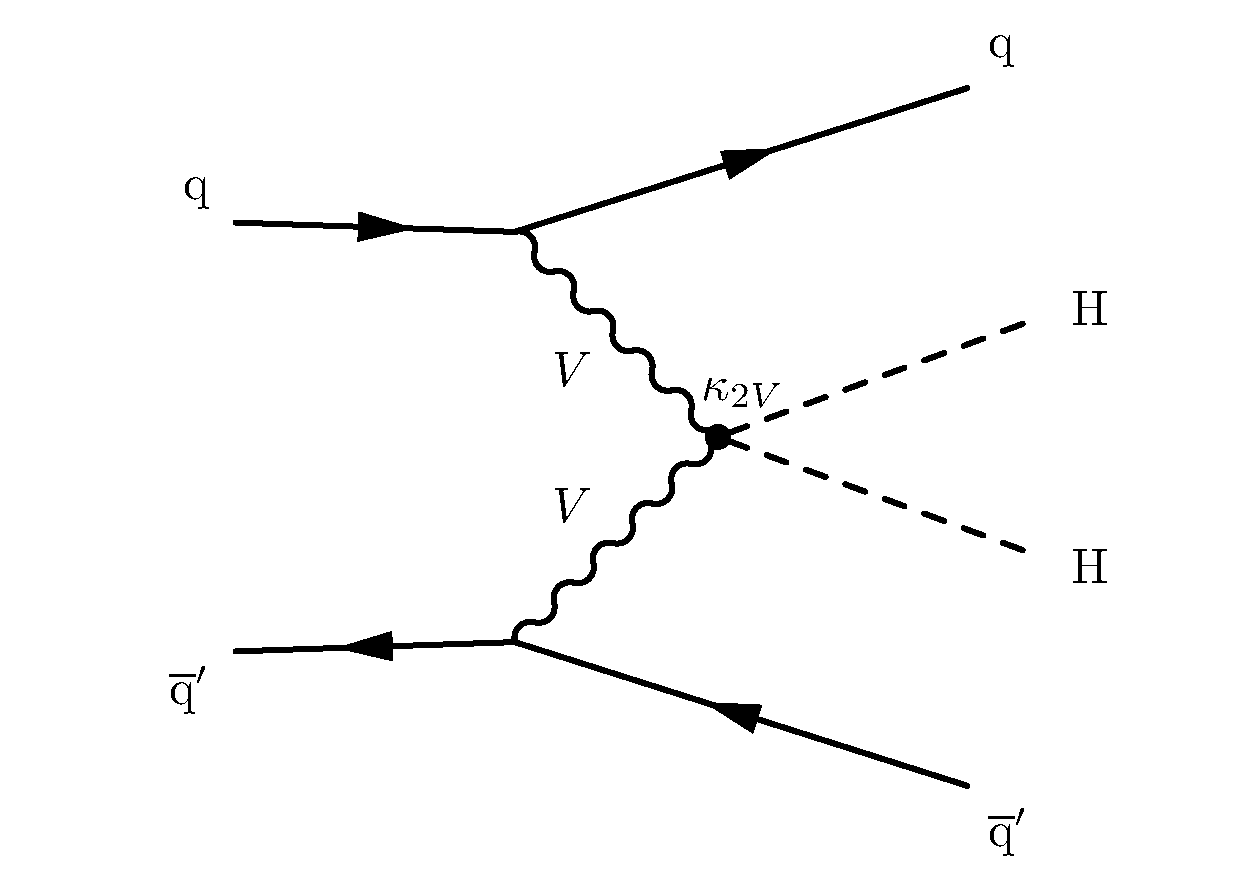
\includegraphics[width=0.45\textwidth]{CMS-PAS-HIG-23-012_Figure_001-e.pdf}
    \caption{
        Diagram for a Higgs boson pair production through gluon fusion (left) and vector boson fusion (right).
        Measuring the rate of Higgs boson pair production enables us to constrain $\lambda$ and $c_{2\PV}$.
        \label{fig:higgs}}
\end{figure}

Without an increase in the center-of-mass collision energy, the improvement in the LHC's sensitivity is limited if we only repeat established searches on larger data sets.
Therefore, innovation and developing new search strategies are necessary.
After the decay to bottom quarks, the next most prominent decay mode of the Higgs boson is its decay to two \PW bosons ($\PH\to\PW\PW$).
This final state is experimentally challenging to identify reliably, especially when the $\PW$ bosons decay to quarks, but can improve the sensitivity to Higgs couplings.

My graduate student Raghav Kansal is the main analyst for a search for Higgs boson pair production through gluon fusion and vector boson fusion in the $\PH\PH\to\bbbar\PW\PW\to\bbbar 4\Pq$ all-hadronic final state.
At high \pt, the decay products of the Higgs boson merge into a single large-radius jet.
This search, now released as a physics analysis summary~[\mycite{CMS-PAS-HIG-23-012}], is the second most sensitive in CMS to the coupling between two vector bosons and two Higgs bosons $c_{2\PV}$.
The data and fitted signal and background distributions are shown for the vector boson fusion category in Fig.~\ref{fig:HH} (left).
While this search is not yet sensitive to the SM production rate, we can exclude many new physics scenarios that would enhance the production rate to this level or above.
The results can also be interpreted as a 95\% CL interval on the $c_{2\PV}$ coupling modifier $\kappa_{2\PV}$---advancing our knowledge of the allowed range for this fundamental parameter.
This search will be included in an upcoming CMS publication combining all Higgs boson pair production searches.


\begin{figure}[htb]
    \centering
    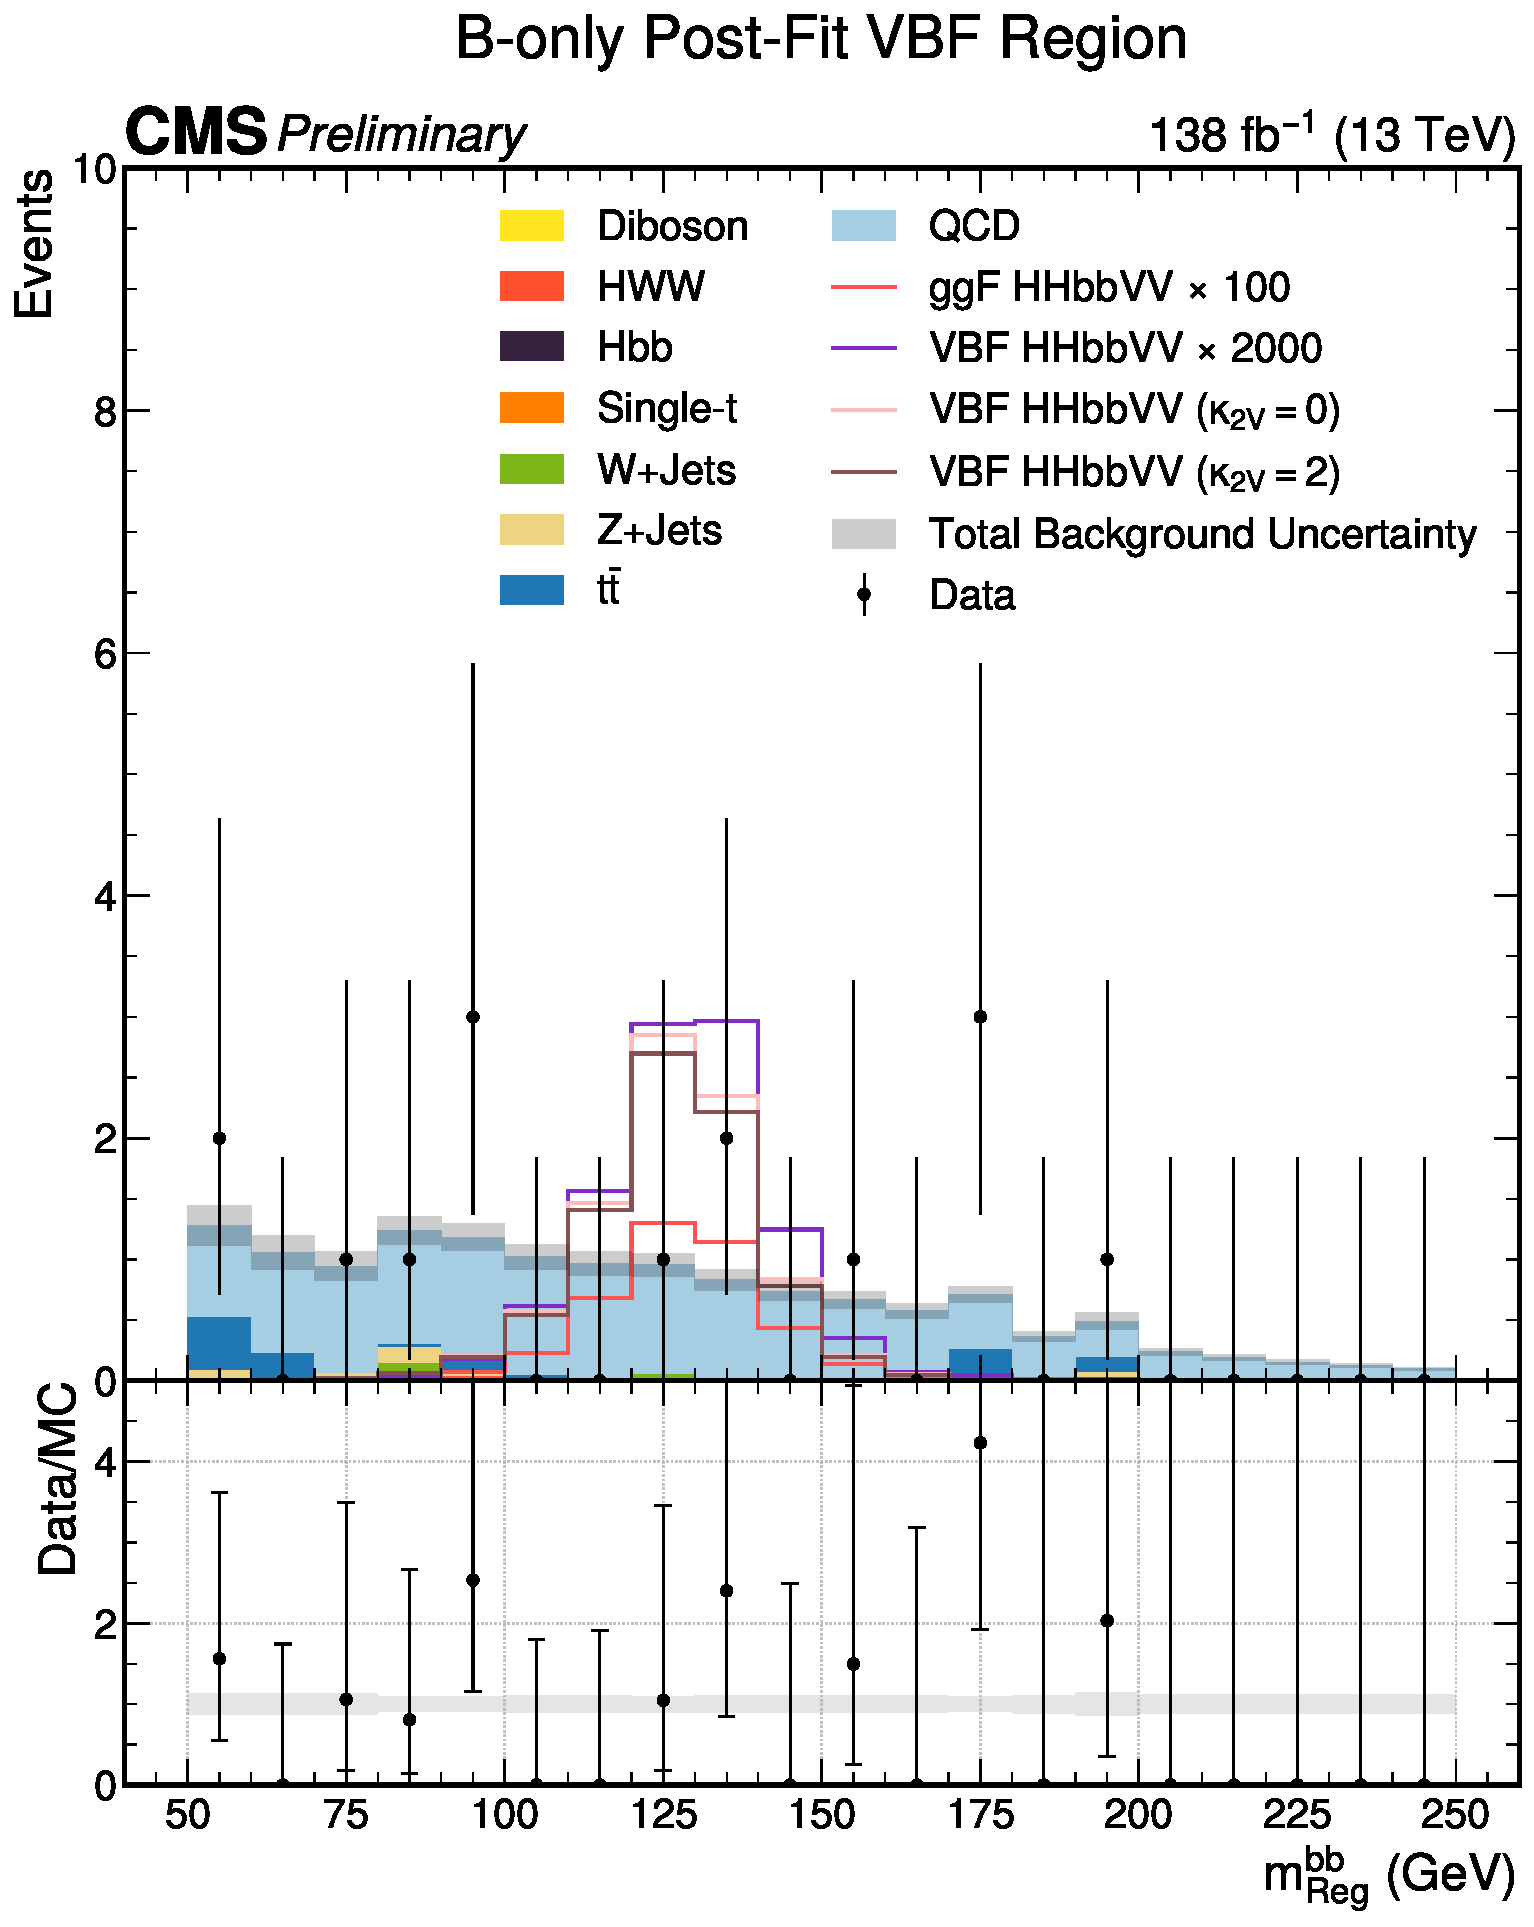
\includegraphics[width=0.35\textwidth]{CMS-PAS-HIG-23-012_Figure_007-b.pdf}
    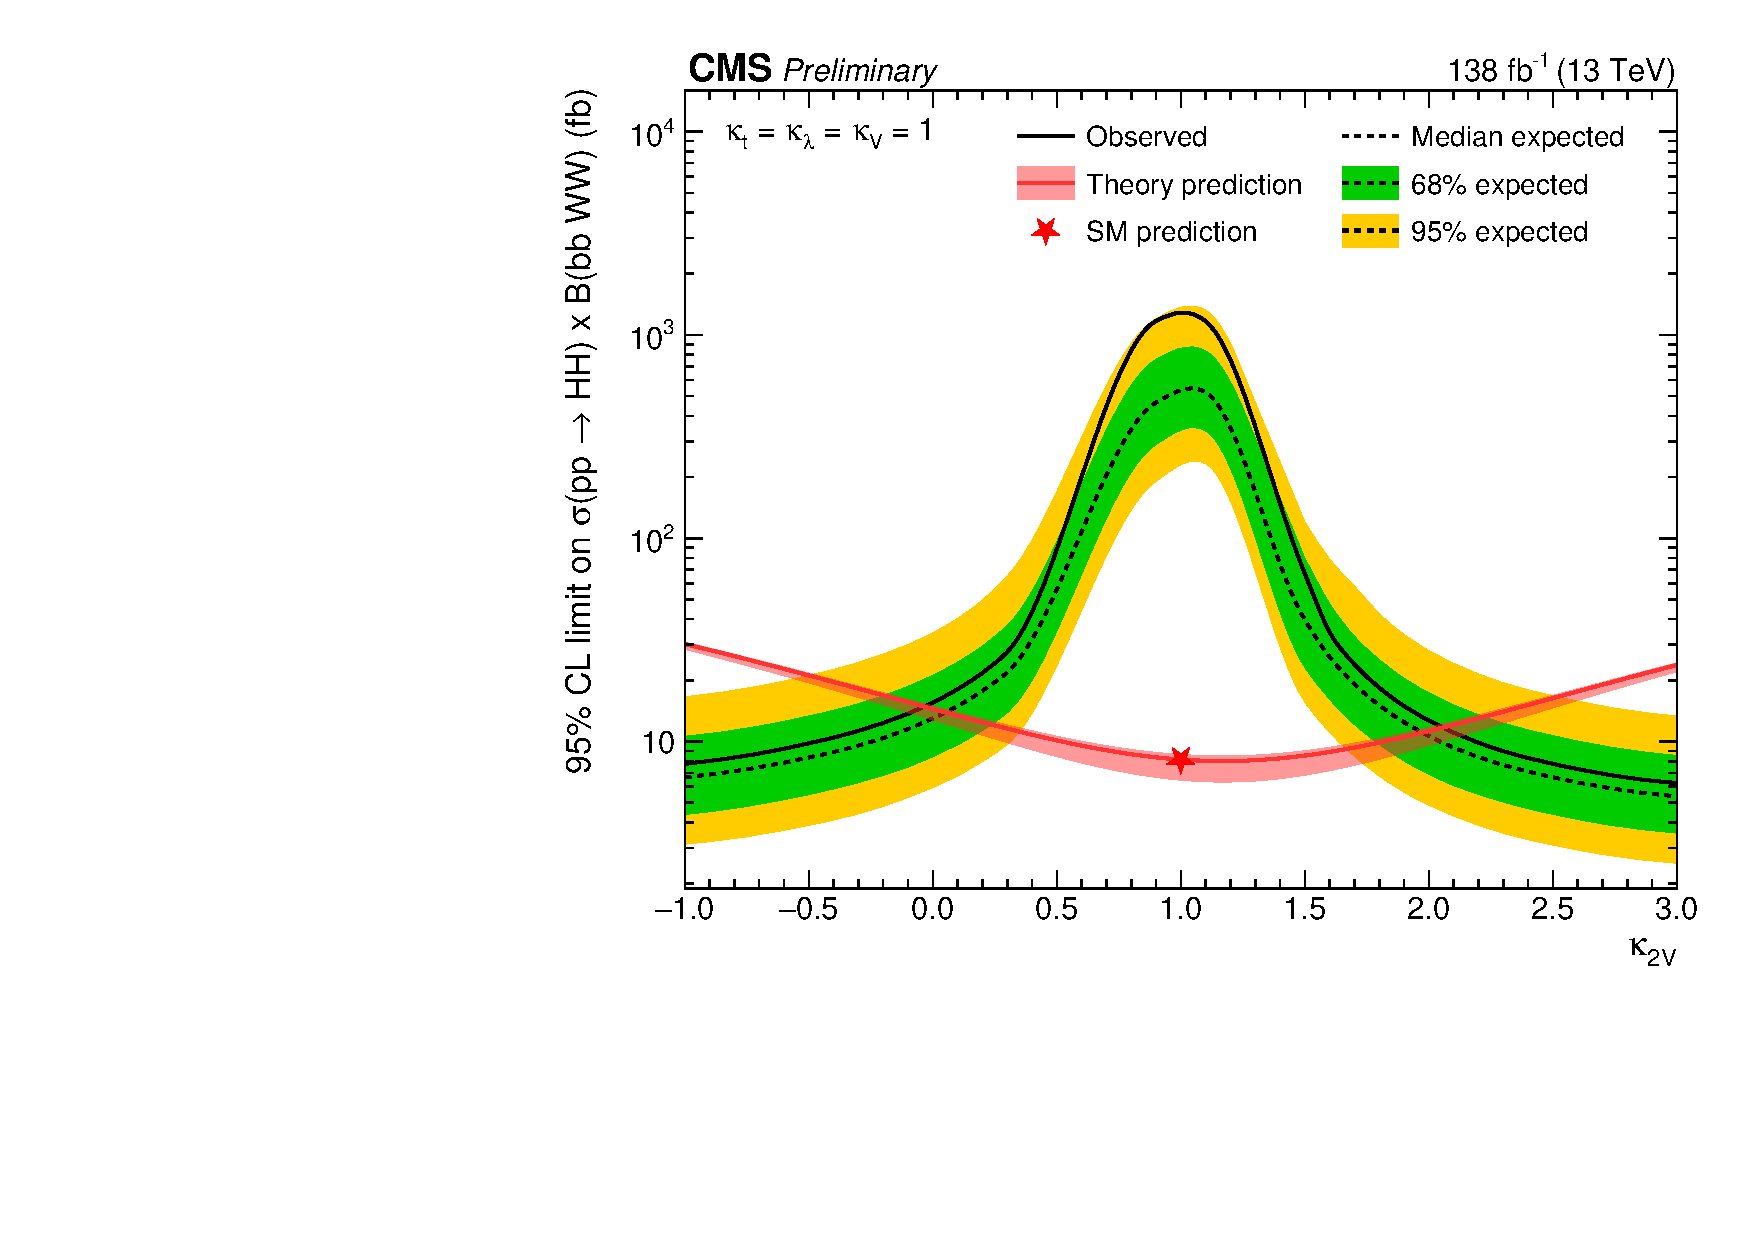
\includegraphics[width=0.50\textwidth]{CMS-PAS-HIG-23-012_Figure_009.pdf}
    \caption{The data and fitted signal and background distributions are shown for the vector boson fusion category in the high-$\pt$ $\PH\PH\to\bbbar\PW\PW\to\bbbar 4\Pq$ search (left).
        The lower panel shows the ratio of the data and the total prediction, with its uncertainty represented by the shaded band.
        The error bars on the data points represent the statistical uncertainties.
        The expected and observed 95\% CL upper limits on the $\PH\PH$ production cross section is shown as a function of the coupling modifier $\kappa_{2\PV}$ (right).
        This search is the second most sensitive to $\kappa_{2\PV}$ from CMS.
        \label{fig:HH}}
\end{figure}


Another graduate student Farouk Mokhtar is the main analyst on a search for single $\PH\to\PW\PW\to\Pq\Pq\ell\nu$ production.
This analysis is on track for publication later this year.
I also contribute to several other ongoing searches for high-\pt Higgs boson production~[\mycite{CMS:2022wqf}, \mycite{CMS-PAS-HIG-21-012}].
This category of my research program is mainly supported by a DOE Early Career Award for ``Real-Time Artificial Intelligence for Particle Reconstruction and Higgs Physics'' (\$750,000 as sole PI, 2020--2025)


\vspace{-1ex}
\subsubsection*{R2. Exotic long-lived particle and jet-based searches}

Many BSM theories predict new particles with long lifetimes for several reasons, including approximate symmetries, small couplings between the LLP and lighter particles, and suppressed phase space available for decays.
For particles moving close to the speed of light, this can lead to macroscopic, detectable displacements between the production and decay points of an unstable particle with a proper decay length $c\tau \gtrsim 10\,\mu$m.
The experimental signatures of LLPs at the LHC are often very different from those of SM processes.
For example, LLP signatures can include deposits of energy inside the calorimeters without associated tracks, stopped particles that decay out of time with collisions, and displaced particle showers in the muon spectrometer.
While the unusual signatures of LLPs offer excellent prospects for their discovery at the LHC, standard reconstruction algorithms may reject events containing LLPs precisely because of their unusual nature.
These atypical signatures can also resemble noise, pileup, or misreconstructed objects in the detector, which may not be accurately modeled in simulations, necessitating data-driven methods to accurately estimate the backgrounds.

During this review period, my graduate students, postdoctoral fellows, and I have been developing a new analysis to search for LLPs using a data sample of $10^{10}$ decays of \PQb hadrons (hadrons that contain bottom quarks), which were recorded and ``parked'' for later analysis by CMS in 2018.
Data parking is a method to evade a major limitation of data collection at the LHC: the computational burden of immediately reconstructing every event.
Instead, raw data from these events were stored without further processing until the data taking run was complete and computational cores were less utilized.
This data set is especially sensitive to a class of models that predict that LLPs are produced in \PQb hadron decays with some small probability.
We expect this work to be finalized and submitted for publication by early next year.
We have also contributed to several other searches for LLPs~[\mycite{CMS:2024bvl}, \mycite{CMS:2024ake}] and boosted dijet resonances~[\mycite{CMS-PAS-EXO-24-007}].

\vspace{-1ex}
\subsubsection*{R3. Novel machine learning for event reconstruction and simulation}

Within the CMS Collaboration, I am the co-convener of the Machine Learning Group, responsible for benchmarking and validating ML methods, coordinating the integration and maintenance of ML software, monitoring the usage of ML in the collaboration, providing consulting, coordinating and centralizing ML training resources for newcomers, fostering ML R\&D, and reviewing publications on novel ML methods.
Under my leadership so far, one paper has been accepted for publication~[\mycite{CMS:2024twn}], three more have been approved and will be submitted to a journal soon, and three additional ones are in preparation.
We have also organized several hackathons, journal clubs, tutorials, and workshops on ML for the collaboration, including the ``CMS ML Hackathon: Anomaly Detection for
Monitoring, Validation, and Discovery'' in July 2024.

Beyond the CMS Collaboration, my research includes developing new ML techniques to improve event reconstruction and simulation in particle physics.
This work is done in collaboration with a relatively small number of coauthors and I made significant technical and writing contributions to these papers.
A novel ML algorithm I helped develop in Ref.~[\mycite{Pata:2021oez}], published in \emph{Eur. Phys. J. C}, uses a GNN to improve the particle-flow (PF) algorithm.
Traditionally, the PF algorithm correlates tracks and calorimeter energy clusters from different detector layers using a set of ad-hoc rules to reconstruct charged and neutral hadron candidates as well as photon, electron, and muon candidates with high efficiency and good energy resolution.
While this approach is effective, it can be brittle and difficult to maintain as detector responses change or detectors get upgraded.
Our ML-based method distills this logic into an algorithm that can be easily updated by retraining on new data or simulation, and gives speed improvements by parallelizing its computation.
During this review period, we have shown this approach can be extended to future proposed colliders and detectors, such as the Compact Linear Collider (CLIC), in work published in \emph{Comm. Phys.}~[\mycite{Pata:2023rhh}].
We also studied the applicability of new hardware for accelerated ML training and inference, like the SDSC Voyager supercomputer composed of AI-specific Intel Habana Gaudi and Goya processors.
This work is facilitated by the NSF award  ``Category II: Exploring Neural Network Processors for AI in Science and Engineering'' (\$5,000,000 for SDSC, 2020--2025) for which I am a co-PI.

My group and I have worked on developing anomaly detection algorithms for particle physics.
An anomaly, in this case, refers to a collection of events that share unusual characteristics that are potentially inconsistent with SM processes, and thus may be related to new BSM particles or interactions.
The methods I've developed are mainly based on autoencoders, a type of ML algorithm trained on SM-like data that compresses then decompresses input data and measures the level of disagreement between the output and the input.
A large discrepancy indicates the data is unlike the SM-like data seen during training, and may be an anomalous signal.
Postdoctoral fellow Melissa Quinnan and I have helped implement this anomaly detection algorithm into data-taking during LHC Run 3~[\mycite{CMS-DP-2023-079}].
Together with an undergraduate student Zichun Hao and graduate student Raghav Kansal, we also developed the first Lorentz-equivariant autoencoder for particle physics~[\mycite{Hao:2022zns}], published in \emph{Eur. Phys. J. C}.


High energy physicists rely heavily on simulation for a wide array of tasks, including data selection, statistical inference, and design optimization for new experiments.
However, the computational demands for simulation of current and next generation experiments are so immense that they have inspired the investigation of generative ML models to decrease simulation time while maintaining fidelity.
Usually, the most computationally intensive step of the simulation is the modeling of the interactions between particles and the detector material.
Some of my work is focused on developing generative ML models using GNNs to improve or speed up this computationally expensive simulation.
Building on our previous work in the 2021 Neural Information Processing Systems (NeurIPS) conference~[\mycite{Kansal:2021cqp}], we have developed a new more efficient transformer-based generative algorithm and comprehensive metrics to compare them, in work published in \emph{Phys. Rev. D}~[\mycite{Kansal:2022spb}].
A workshop paper describing the improved efficient algorithm was also accepted to the NeurIPS Workshop on Machine Learning for the Physical Sciences in 2023~[\mycite{Li:2024xpw}].
The software related to this work was released as a public library called JetNet, described in a publication in \emph{J. Open Source Softw.}~[\mycite{Kansal:2023joss}].

A common thread throughout this work is developing open, public scientific data sets~[\mycite{Chen:2021euv}] and sharable AI models following the findable, accessible, interoperable, and reusable (FAIR) principles~[\mycite{Duarte:2022job}].
These principles are significant because they enable more reproducible science, greater access to a larger community of researchers, and support educational efforts.
This work was partially funded by a DOE award \href{https://fair4hep.github.io}{``FAIR4HEP: FAIR Framework for Physics-Inspired AI in High Energy Physics''} (\$2,250,000 total, \$450,000 for UCSD, 2020--2023) on which I was a co-PI.

\vspace{-1ex}
\subsubsection*{R4. Accelerated machine learning for trigger and computing}

In the next phase of the LHC, the instantaneous luminosity will increase by a factor of five and the CMS detector will become more complex, producing up to hundreds of terabytes of data per second.
This avalanche of data must be filtered down by several orders of magnitude by the real-time, hardware-based trigger system within microseconds using field-programmable gate arrays (FPGAs).
To meet this challenge, my research focuses on developing new ultra-low-latency AI techniques trained to reconstruct, identify, and preserve these precious collisions.
This work has broader impacts for many disciplines, including multimessenger astronomy, neutrino physics, neuroscience, and microscopy~[\mycite{Deiana:2021niw}, \mycite{Duarte:2022efficient}].

I contributed to the design, implementation, and evaluation of real-time AI algorithms on FPGAs for the LHC trigger.
My key contribution is the creation and continued development of \texttt{hls4ml}~[\mycite{Duarte:2018ite}], a generic tool allowing scientists to translate ML algorithms into FPGA firmware.
In Ref.~[\mycite{Odagiu:2024bkp}], we developed new implementations of deep set and graph neural networks in FPGAs for jet tagging in the LHC trigger, and compared their performance.
In Ref.~[\mycite{Shenoy:2023ros}], we developed a differentiable approximation to the Earth mover's distance in order to train a better autoencoder for data compression.
% For all the above work, I oversaw the development and validation of these implementations and cowrote the publications.

As more physics reconstruction and simulation algorithms turn to ML-based approaches, there is a need to scale up and accelerate the inference of large ML models in order to run them on billions of collision events in distributed computing workflows.
The goal is to enable the use of alternative processors, alongside traditional CPUs, that are better adapted to highly parallelizable ML inference workloads in a scalable way.
With coauthors, we developed a new framework of ``ML inference as a service'' for particle physics~[\mycite{Duarte:2019fta}], in which heterogeneous computing elements, including graphics processing units (GPUs), FPGAs, and AI-targeted application-specific integrated circuits (ASICs), can be flexibly composed and used with in tandem with CPUs.
I contributed to the integration of these workflows into the CMS computing framework, which is documented in a paper accepted by \emph{Comput. Softw. Big Sci.}~[\mycite{CMS:2024twn}].

This work is also supported by my DOE Early Career Award and the \href{https://a3d3.ai}{``NSF Harnessing the Data Revolution (HDR) Institute for Accelerated AI Algorithms for Data Driven Discovery (A3D3)''} (\$15,000,000 total, \$675,600 for UCSD, 2021--2026) focused on the domains of multimessenger astronomy, neuroscience, and particle physics.
For this Institute, I am a key personnel, the UCSD institute PI and co-chair of the Equity and Career Committee.
I also coordinate the Targeted Systems group,
Some of this work is also supported by a DOE Award for ``Real-time Data Reduction Codesign at the Extreme Edge for Science'' (\$750,000 total, \$225,000 for UCSD, 2021--2024), on which I am a co-PI.
\vspace{-1ex}
\subsection*{Mentorship}

My research group has grown substantially to include two postdoctoral fellows, Dr. Melissa Quinnan and Dr. Daniel Diaz, seven physics graduate students, Raghav Kansal (Ph.D. year 5), Farouk Mokhtar (Ph.D., year 4), Anthony Aportela (Ph.D., year 4), Daniel Primosch (Ph.D., year 4), Russell Marroquin Solares (Ph.D., year 2), Zihan Zhao (Ph.D., year 2), and Haoyang (Billy) Li (Ph.D., year 2), and more than 10 undergraduate student researchers.
I also supervise or co-supervise several Computer Science and Engineering (CSE) and Electrical and Computer Engineering (ECE) graduate students: Olivia Weng (CSE Ph.D., year 4, co-supervisor with Ryan Kastner), and Steven Tsan (CSE M.S., year 2, sole supervisor).
With my support, several of these students have received significant awards and funding.
For example, Raghav Kansal was awarded an LHC Physics Center (LPC) Graduate Scholarship, Daniel Diaz was named an LPC Distinguished Researcher, and Russell was awarded a Western Advanced Training for Computational High-Energy Physics
(WATCHEP) fellowship.
From the School of Physical Sciences, Emily Pan, Jason Weitz, Simon Poon, Mengke (Michael) Zhang received Dean's Undergraduate Excellence Awards in 2023--2024, and Anni Li, Rohan Shenoy, and Thomas Sievert received Dean's Undergraduate Excellence Awards in 2022--2023.
Many other undergraduate students have also received awards and funding from the UCSD TRELS program, Undergraduate Research Hub, the Division of Physical Sciences Undergraduate Research Award, and NSF IRIS-HEP.
A great deal of the work done by undergraduates in my group has led to publications or conference papers.
This includes work led by Rohan Shenoy on improved autoencoder training~[\mycite{Shenoy:2023ros}]Anni Li on simulation~[\mycite{Li:2024xpw}] and Zichun Hao on Lorentz-equivariant autoencoders for anomaly detection~[\mycite{Hao:2022zns}], and Jason Weitz and Dmitri Demler on neural architecture codesign~[\mycite{McDermott:2023neural}].

My graduate students Anthony Aportela and Russell Marroquin Solares received HEPCAT and WATCHEP fellowships, respectively.
The HEPCAT fellowship is supported by a DOE award (\$3,700,000 total, \$110,000 for UCSD so far, 2021--2026), which aims to support and train the next generation of HEP instrumentation researchers.
For this award, I am Key Personnel and lead the \href{https://hepcat.ucsd.edu/topical-groups/tg7-ai-ml-for-detectors-2/}{Topical Group on AI/ML for detectors}.
The WATCHEP fellowship is also supported by a DOE award (\$2,000,000 total, \$440,00 for UCSD, 2022--2027), which trains students on computational topics in experimental particle physics.

% I devoted substantial effort to securing external funding by submitting several 
\vspace{-1ex}
\subsection*{Teaching}

My teaching approach is to foster an inclusive, welcoming learning environment and promote active learning through evidence-based methods.
I also strive to provide sufficient scaffolding through lower-stakes, incremental assignments.
For example on homework assignments, half of the grade is earned through a draft, and the other half is earned through revisions to reinforce the concepts that students may have misunderstood.
I also use ``exit tickets'' and surveys to collect feedback on the course structure, difficulty of projects, and appropriateness of the assessments.

During this review period, I have focused on developing new computational physics courses and updating existing ones.
I have created a new introductory graduate and upper-division undergraduate course, currently taught as a special topics course called Physics 139/239: Machine Learning in Physics.
The course structure consists of weekly lectures on conceptual topics, e.g. statistics, linear algebra, scientific data set exploration, feature engineering, (stochastic) gradient descent, neural networks, and unsupervised learning.
Students learn key concepts in data science and machine learning, including selecting and preprocessing data, designing machine learning models, evaluating model performance, and relating model inputs and outputs to the underlying physics concepts.
They apply these methods to the domains of collider physics, neutrino physics, astronomy, and others.
In addition to hands-on programming-based homework assignments, the final project for the course is an open-ended group research project to reproduce the results of an ML in physics research article, with intermediate checkpoints to provide feedback.
A midterm assignment to propose the project is also required.
The projects use real, open scientific datasets, including those shown in Fig.~\ref{fig:teaching} (right).
The use of real data sets communicates to students that they are doing publication-quality work at the interface of machine learning and physics.
The course acts as a bridge between theory and practice in research, providing authentic learning experiences to prepare students for professional work and advanced academic research.
Throughout the two quarters, students completed final group projects on galaxy image classification, gravitational wave noise reduction, neutrino event identification, temperature field prediction, superconductor property prediction, and more.

I also revamped Physics 141/241: Computational Physics I: Probabilistic Models and Simulations and Physics 142/242: Computational Physics II: PDE and Matrix Models.
I helped procure the availability of modern campus computing resources using the UCSD JupyterHub Data Science and Machine Learning Platform (DSMLP).
I showed students how to use modern computing tools like Jupyter, Git, Docker, Numpy/Numba, and Kubernetes for exploratory programming, writing accelerated vectorized code, collaboration and version control, creating reproducible environments, and orchestrating jobs over large clusters.
The students gave positive feedback on gaining this experience, finding the skills transferable to computational research and job opportunities.

Finally, I also co-taught a new graduate course developed with Prof. R. Sekhar Chivukula, Physics 239: Computational Methods in Collider Physics, covering beyond the SM physics, Monte Carlo event generators, detector simulation, and ML methods for data analysis.
The goal of the course is to give graduate students an ``end-to-end'' view of the process from theoretical prediction to experimental constraints.


Overall, I received good ratings in the CAPE and SET evaluations for the new and updated courses.
According to CAPE evaluations, for the new Physics 139/239 (Winter 2023) and updated Physics 141/241 (Spring 2023), 75\% and 86.4\% recommended the course and 100\% and 95.2\% recommended me as the instructor, respectively.
According to SET evaluations, for the updated Physics 142/242 (Winter 2024) and new Physics 139/239 (Spring 2024), students gave scores of 4.93/5.00 and 4.67/5.00 for student learning, 4.74/5.00 and 4.53/5.00 for course structure, and 4.51/5.00 and 4.43/5.00 for class environment.


\begin{figure}[htb]
    \centering
    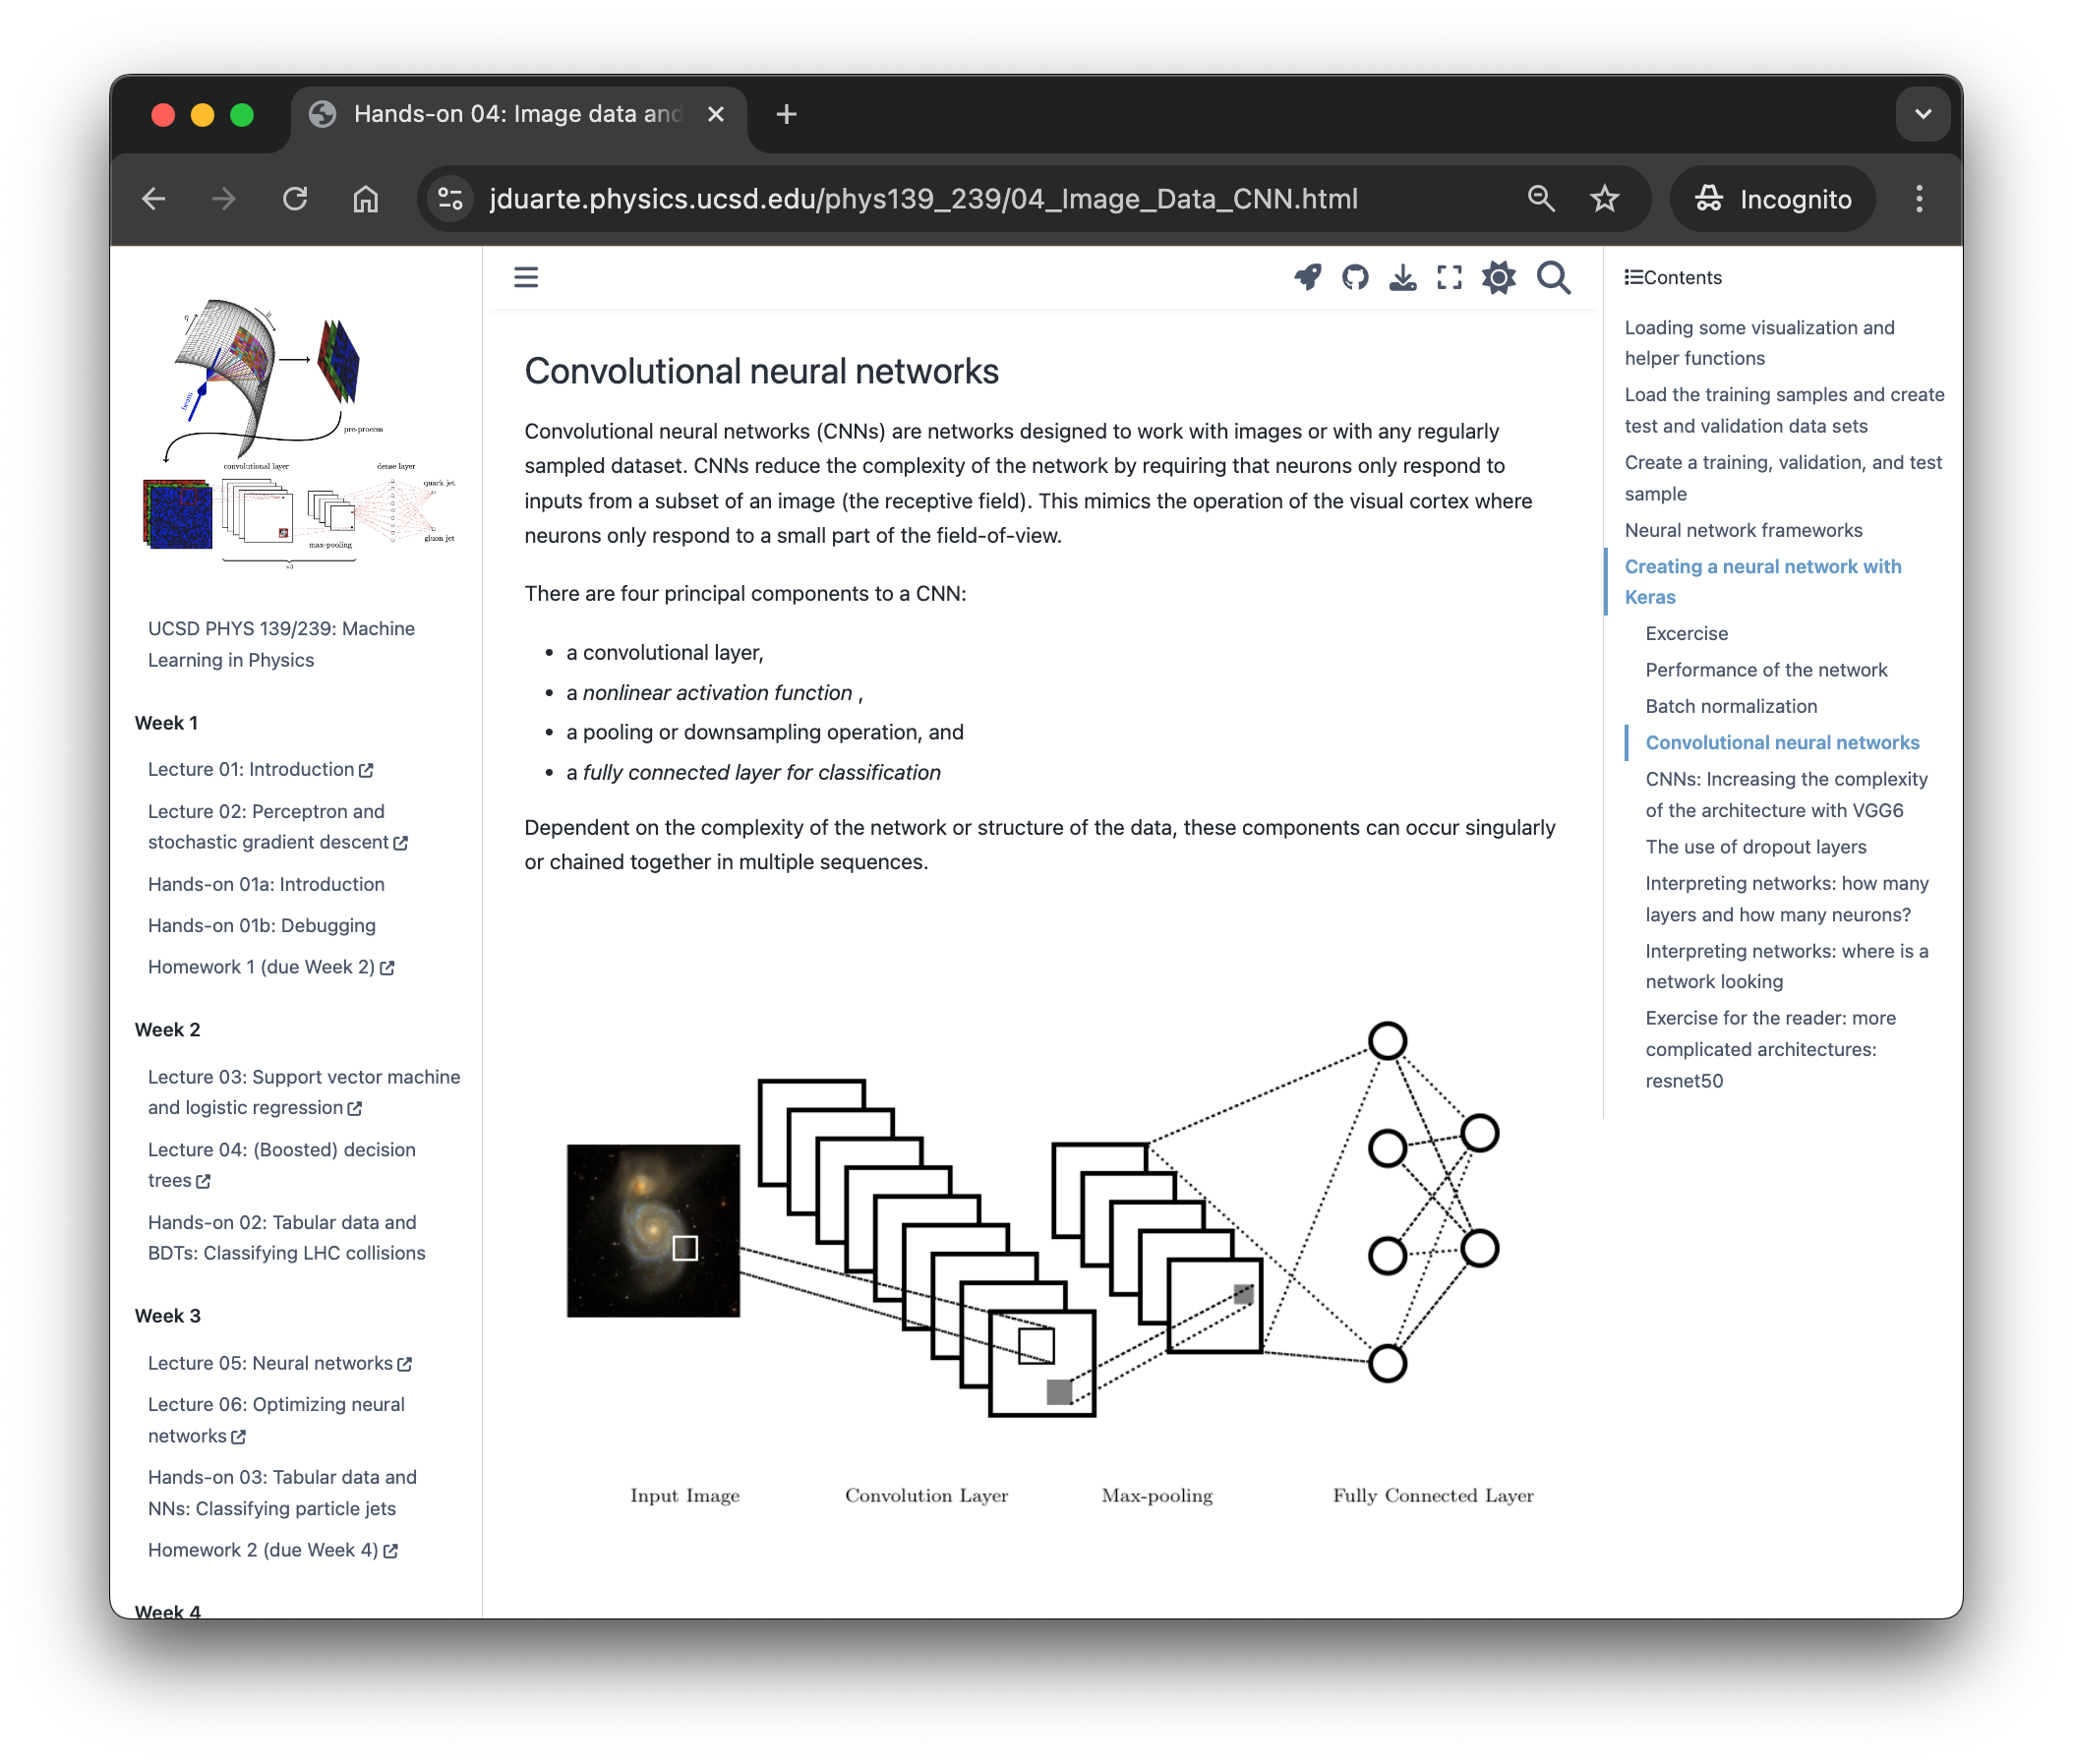
\includegraphics[width=0.4\textwidth]{jupyterbook.png}
    \includegraphics[width=0.55\textwidth]{phys141_data.pdf}
    \caption{Demonstration of the Jupyter Book format (left).
        The code is executable and renders in the browser.
        Visualizations of data sets used in Physics 139/239: (a) high-energy collider physics data consisting of simulated particle jets from the CMS experiment for identifying Higgs bosons, (b) astrophysical time-series data consisting of gravitational wave transient events maintained by the LIGO/Virgo/KAGRA collaboration, and (c) neutrino physics data containing simulated neutrinos interacting in a liquid argon time projection chamber (right).
        \label{fig:teaching}}
\end{figure}

\vspace{-1ex}
\subsection*{Service}

Beginning in 2022, I served as the Physics Department representative to the Equity in Graduate Education (EGE) Consortium, formerly known as the California Consortium for Inclusive Doctoral Education (C-CIDE).
I am also the Physics Department representative for the Mentoring Project.

I have served as a peer reviewer for \emph{J. High Energy Phys.}, \emph{Phys. Lett. B}, \emph{Phys. Rev. D}, \emph{Phys. Rev. Research}, \emph{Eur. Phys. J. C}, \emph{Comput. Softw. Big Sci.}, and \emph{Nucl. Instrum. Methods Phys. Res. A}, and \emph{Applied Optics}, and as a Guest Associate Editor for \emph{Front. Big Data} and \emph{Front. AI}.
I have also reviewed for the Neural Information Processing Systems (NeurIPS) Conference in 2023.
I have served as an external reviewer of grant applications for the NSF and DOE.
I was part of the Scientific Organizing Committee for the Fast Machine Learning for Science Workshop in 2022, 2023, and 2024.
I was also a member of the Scientific Program Committee (Track 2: Data Analysis - Algorithms and Tools) for the 22nd International Workshop on Advanced Computing and Analysis Techniques in Physics Research (ACAT) in 2024.

\vspace{-1ex}
\subsection*{Equity, Diversity, and Inclusion}

As a faculty member, I have led Equity, Diversity, and Inclusion (EDI) initiatives, especially promoting equitable graduate admissions.
I was recognized for these contributions by a UCSD Inclusive Excellence Award in 2023.
As key personnel of the NSF HDR A3D3 Institute, I co-chair the Equity and Career Committee.
One of my main contributions in this role was the conception and execution of the A3D3 Postbaccalaureate Research Fellowship.
This one-year fellowship is intended to increase research opportunities for URM groups in STEM, including African American/Black, Chicanx/Latinx, Native American/Alaska Native, Native Hawaiin/Pacific Islander, and Filipinx scientists.
In particular, the program is intended as a bridge to help students with a lack of access to research opportunities gain experience while being supported with mentoring and professional development activities (like technical writing seminars), in order to be more competitive for graduate study or industry positions.
In our first three years (2022--2025), twelve postbaccalaureate fellows have been recruited to conduct research at institutions across the country including UCSD.

I am the lead PI on a Cottrell Scholars Collaborative titled ``Hidden Figures in Physics and Astronomy'' (\$25,000, 2023--2025) funded by the Research Corporation for Science Advancement.
The aim of this project is to create a database of URM scientists in physics and astronomy, and to develop a series of educational modules for college students to learn about the contributions of URM scientists to these fields.
A preliminary version of the database is available at\\\href{https://hiddenfigs.github.io}{hiddenfigs.github.io}.

I have also mentored students ranging from high school to graduate school participating in the SDSC MAP, UCSD EXPAND, UCSD ENLACE, UCSD STEMULATE, Cal-Bridge, CERN REU, IRIS-HEP fellowship, APS National Mentorship, and US CMS Mentorship programs.
Many of these programs specifically aim to provide opportunities for URM students in STEM.
I am a faculty co-chair of APS Conference for Undergraduate Women and Gender Minorities in Physics (CU*iP) planned to take place in January 2025 at UCSD.
Finally, I contribute to department-level outreach activities, for example, as an exhibitor for the Physics Department and my lab at the \href{https://www.barriologansae.com/}{Barrio Logan Science \& Art Expo} on Saturday, April 16, 2022.

\vspace{0.1in}
\includegraphics{signature.pdf}\\
\indent\indent Javier M. Duarte\\
\indent\indent \today

\end{document}
